\documentclass[a4paper,12pt]{book}
\usepackage[numbers]{natbib}
\bibliographystyle{plainnat}
\usepackage{graphicx}
\usepackage{verbatim}
\usepackage{color, colortbl}
%\usepackage[pdftex]{color}
\usepackage{hyperref}
\usepackage[utf8]{inputenc}
\setcounter{tocdepth}{2}
\usepackage{alltt}
\usepackage{amsmath}
\usepackage{amssymb}
\usepackage{amsfonts}
\graphicspath{{./images/}}
\usepackage{txfonts}   %%does not work on Windows
\usepackage{dsfont}
\usepackage[toc,page]{appendix}
\usepackage{dirtree}
%
\newcommand{\NAME}{AQUAgpusph }
\newcommand{\VERSION}{1.5.03 }
\newcommand{\rc}{\\[0.2 in]}
\newcommand{\rcc}{\\[0.3 in]}
\newcommand{\rccc}{\\[0.4 in]}
% \newcommand{\bs}[1]{\boldsymbol{#1}}
\newcommand{\bs}[1]{\pmb{#1}}
\newcommand{\SPHint}{\int_{\bs{y} \in \Omega}}
\newcommand{\SPHboundint}{\int_{\bs{y} \in \partial \Omega}}
\newcommand{\gradient}{\nabla}
\newcommand{\divergence}{\mbox{div}}
\newcommand{\laplacian}{\bigtriangleup}
\newcommand{\dsty}{\displaystyle}
\newcommand{\sph}[1]{\langle {#1} \rangle}
%
\author{JL Cercos-Pita $<$jl.cercos@upm.es$>$}
\title{\vspace{-2em}
\NAME- \VERSION.\rcc
\textbf{Developers guide}}
\date{\today\\[4.0 in]
\begin{figure}[h!]
  \centering
  
\includegraphics[width=0.2\textwidth]{CC_88x31}
\end{figure}
}
%
\setlength{\parindent}{0em}
%
% \usepackage{anysize}
% \marginsize{1.5cm}{1cm}{1cm}{1cm}
\usepackage[a4paper,inner=1.5cm,outer=1.5cm]{geometry}
%
\usepackage{fancyhdr}
\pagestyle{fancyplain}
% Pages header and foot
\lhead{}
\rhead{\NAME- \VERSION developers guide}
\lfoot{JL Cercos-Pita}
\cfoot{\url{http://canal.etsin.upm.es}}
\rfoot{\thepage}

%%%%%%%%%%%%%%%%%%%%%%%%%%%%%%%%%%%%%%%%%%%%%%%%%%%%%%%%%%%%%%%%%%%%%%%%%%%%%%%%%%%%
\begin{document}

% -------------------------------
% Title and summary
% -------------------------------
\maketitle
\thispagestyle{empty}
%
\newpage
\tableofcontents
\newpage
\newpage

% -------------------------------
% Introduction items
% -------------------------------
\chapter{Introduction}
\label{s:introduction}
%
\section{About \NAME}
%
\NAME (Another QUAlity GPU-SPH) is a free CFD software licensed under GPLv3,
and developed by J.L. Cercos-Pita as part of his PhD at CEHINAV-UPM group
\footnote{Model Basin Research group, Technical University of Madrid (UPM),
\url{http://canal.etsin.upm.es}}. \NAME is based on Lagragian meshfree SPH
(Smoothed Particles Hydrodynamics) method.\rc
%
\NAME has been accelerated with OpenCL, that allows you to execute it over
CPU based platforms, over GPUs based platforms, and eventually, over every platform
developed in the future adapted to the OpenCL standard. For the moment the simultaneous
use of several platforms in the same simulation is not supported.\rc
%
The code has been widely validated, used and documented in several publications, for
instance \citet{Maciaetal_PTP_2012} where boundary integrals are tested or
\citet{perezrojas_cercos_stab12} where SPHERIC benchmark test case number 9 was simulated.
Some examples provided within the package have been studied in these publications.\rc
%
\NAME has been designed for UNIX like operative system, and tested on GNU/Debian Linux distributions.
%
For the moment no ports has been developed for Windows or Mac operative systems.
%
\NAME has been developed in C\texttt{++} and OpenCL\footnote{OpenCL is so quite similar to C}. Also Python extensions has been developed.
%
\section{License notes}
%
\NAME is free software: you can redistribute it and/or modify
it under the terms of the GNU General Public License as published by
the Free Software Foundation, either version 3 of the License, or
(at your option) any later version.\rc
%
\NAME is distributed in the hope that it will be useful,
but WITHOUT ANY WARRANTY; without even the implied warranty of
MERCHANTABILITY or FITNESS FOR A PARTICULAR PURPOSE.  See the
GNU General Public License for more details.\rc
%
You should have received a copy of the GNU General Public License
in 'LICENSE' file with \NAME package. If not, see
\url{http://www.gnu.org/licenses/}.
%
\section{Objectives of the present document}
%
This document has been created aiming to provide a tool that allows the \NAME developers to know:
%
\begin{enumerate}
	\item The structure of \NAME source code.
	\item The location of the source codes and helper files.
	\item The entry points to the main parts of AQUAgpusph
\end{enumerate}
%
This document is trying to complement the Doxygen documentation.
%
Such documentation can be get, either building it with CMake (see the user manual) or in the following web page (corresponding to the last stable \NAME package):\rc
%
\url{http://canal.etsin.upm.es/aquagpusph/doc/doxygen/stable}
%
\section{Required background}
%
The background required for the developers depends on the section of the code to be read/modified:
%
\begin{enumerate}
	\item The kernel of \NAME is written C\texttt{++}.
	\item The computational tools are written in OpenCL.
	\item The examples are built using XML files.
	\item Also Python extension may be used in some examples.
	\item The documentation (this document as well as the developers guide) is written in \LaTeX.
	\item The configuration and compilation is carried out with CMake.
\end{enumerate}

Also, depending on the modifications to be done, some background in CFD, and more specifically in SPH, may be required.
%

% -------------------------------
% AQUAgpusph structure
% -------------------------------
\chapter{\NAME strcuture}
\label{s:structure}
%
\section{General}
\label{ss:structure::general}

\NAME package is divided in several parts:
%
\begin{enumerate}
	\item \NAME kernel.
	\item Computational tools.
	\item Helper tools.
	\item Examples.
	\item Documentation.
	\item CMake configuration and compiling files.
\end{enumerate}

\section{Kernel}
\label{ss:structure::kernel}
%
The kernel on \NAME is basically the main program which will be executed in the CPU.
%
When it is launched the following operations will be owned by the main program:
%
\begin{enumerate}
	\item The input XML files loading.
	\item The computational device setup.
	\item The OpenCL kernels loading.
	\item The OpenCL codes execution querying (this codes will be ran in the computational device).
	\item The Python scripts loading and executing.
	\item The output files writing.
\end{enumerate}
%
The source code files are placed in both \textbf{src/} and \textbf{include/} package folders.\rc
%
The kernel is divided in two main parts, widely denominated ``host'' and ``server''. Such division can be appreciated in figure \ref{fig:structure::kernel:generalDiagram}.
%
\begin{figure}[ht!]
  \centering
  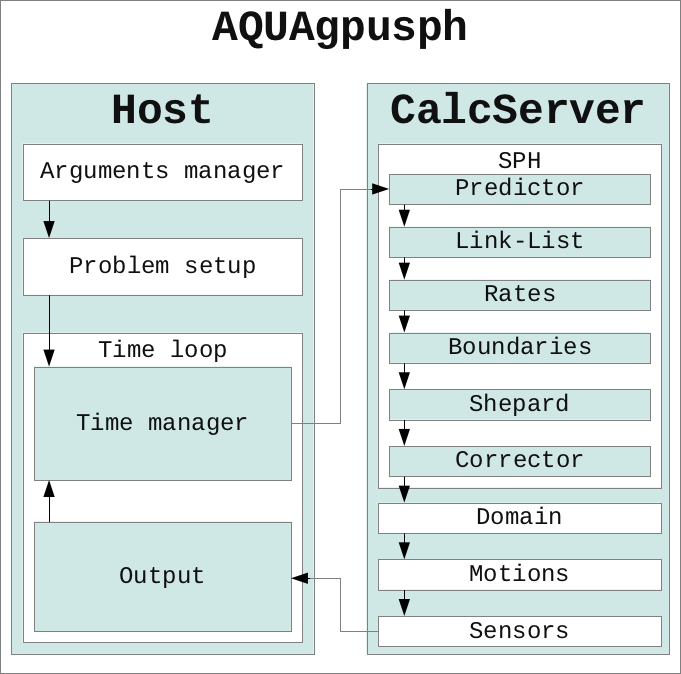
\includegraphics[width=0.7\textwidth]{GeneralDiagram}
  \caption{General \NAME flux diagram}
  \label{fig:structure::kernel:generalDiagram}
\end{figure}
%
Developers interested in the ``host'' side, mainly responsible of the input and output, may start with the file \href{http://canal.etsin.upm.es/aquagpusph/doc/doxygen/stable/df/d0a/main_8cpp.html}{\textbf{src/main.cpp}}.\rc
%
Developers interested in the ``server side'', designed to control the simulation querying the OpenCL codes execution, may start with the class \href{http://canal.etsin.upm.es/aquagpusph/doc/doxygen/stable/dd/d66/classAqua_1_1CalcServer_1_1CalcServer.html}{\textbf{CalcServer}}.\rc
%
You can learn more about the source code files location and objective in the Doxygen documentation:\rc
%
\url{http://canal.etsin.upm.es/aquagpusph/doc/doxygen/stable/files.html}
%
\section{Computational tools}
\label{ss:structure::opencl}
%
The computational tools are OpenCL codes placed in \textbf{resources/OpenCL} folder.
%
These codes are running in the computational device, and therefore are widely related with the kernel ``server'' side tools.\rc
%
You can learn more about the OpenCL codes in the Doxygen documentation:\rc
%
\url{http://canal.etsin.upm.es/aquagpusph/doc/doxygen/stable/files.html}\rc
%
It should be mentioned that, being these codes the provided with \NAME package, they can be replaced by other ones for specific simulations just setting it in the input XML files.
%
\section{Helper tools}
\label{ss:structure::tools}
%
With \NAME package several helper tools are provided.
%
These tools are placed in the \textbf{tools/} folder.\rc
%
Probably the most important tools are placed in \textbf{tools/aquagpusph\_preprocessing}, being the particles generators.
%
The generators are scripts that can read a mesh and generate the boundary particles in the mesh and the fluid ones inside it.
%
\section{Examples}
\label{ss:structure::examples}
%
The examples are placed in the \textbf{examples/} folder.
%
The examples available depends on whether the 2D or the 3D version of \NAME is built.
%
In \NAME package each example has its files divided in 2 folders, namely:
%
\begin{enumerate}
	\item \textbf{examples/\textit{example\_name}}
	\item \textbf{examples/cMake/\textit{example\_name}}
\end{enumerate}
%
where \textit{example\_name} is replaced by the example folder name.
%
In the first folder the files which does not require any specific configuration are placed, while in the latter folder the files which require to be modified according to the cMake configuration are placed.
%
When the examples are built, all the files (conveniently configured) are placed in the first folder.\rc
%
In the built examples following files may be found:
%
\begin{enumerate}
	\item Create.py: Python script to generate the particles input file.
	\item Fluid.dat: Particles file generated by Create.py.
	\item Main.xml: Main input XML file, it is just including other XML files.
	\item Settings.xml: General program settings:
	\url{http://canal.etsin.upm.es/aquagpusph/doc/doxygen/stable/d8/dfe/structAqua_1_1InputOutput_1_1ProblemSetup_1_1sphSettings.html}
	\item Time.xml: Simulation time flow options:
	\url{http://canal.etsin.upm.es/aquagpusph/doc/doxygen/stable/de/d49/structAqua_1_1InputOutput_1_1ProblemSetup_1_1sphTimingParameters.html}
	\item SPH.xml: Physics simulation parameters:
	\url{http://canal.etsin.upm.es/aquagpusph/doc/doxygen/stable/d6/d08/structAqua_1_1InputOutput_1_1ProblemSetup_1_1sphSPHParameters.html}
	\item GhostParticles.xml: Ghost particles boundaries (just when Ghost particles boundary condition is applied):
	\url{http://canal.etsin.upm.es/aquagpusph/doc/doxygen/stable/d5/d89/classAqua_1_1InputOutput_1_1ProblemSetup_1_1sphGhostParticles.html}
	\item Fluids.xml: Fluids physics properties:
	\url{http://canal.etsin.upm.es/aquagpusph/doc/doxygen/stable/d7/da8/structAqua_1_1InputOutput_1_1ProblemSetup_1_1sphFluidParameters.html}
	\item Movements.xml: Motions to be parsed:
	\url{http://canal.etsin.upm.es/aquagpusph/doc/doxygen/stable/dd/df7/classAqua_1_1InputOutput_1_1ProblemSetup_1_1sphMoveParameters.html}
	\item Move/6DOF.xml: Specific motion type parameters.
	\item Move/move.py: Python script which controls the solid motion (just in Python script controlled motions).
	\item run.sh: Helper running script, type ``./run.sh --help'' in the example folder to learn more.
\end{enumerate}
%
Some other files may be found, for instance, to plot the results in real time, or to load the prescribed solid motions.\rc
%
\textbf{Main.xml} file is also including the shared XML file \textbf{resources/OpenCLMain.xml}, which is automatically setting all the computational tools discussed in the section \ref{ss:structure::opencl}.
%
\section{Documentation}
\label{ss:structure::doc}
%
The documentation files, which include the user manual, the developers guide and the Doxygen documentation, are placed in the folder \textbf{doc/}.\rc
%
In \NAME it is expected that the Doxygen documentation is built using cMake, so please do not try to build it manually.\rc
%
Regarding the user manual and the developers guide, \NAME is providing already compiled version of them, however they can be edited and recompiled using the \textbf{buildPDF.sh} script provided with each one.
%
\section{CMake}
\label{ss:structure::cmake}
%
All the files called ``\texttt{CMakeLists.txt}'', ``\texttt{*.cmake}'', or 
included in a ``cMake'' folder are designed to let CMake to configure the 
package for the build and installation process.
%
More specifically, the files called ``\texttt{CMakeLists.txt}'' are the ones 
where the instructions for CMake are written, while the other ones are 
templates that CMake is conveniently reading and editing.


% -------------------------------
% Directory tree
% -------------------------------
\begin{appendices}
\chapter{Directory tree}
%
Following all the files provided with \NAME package, with its location, is 
shown.
%
The files autogenerated during the configuration, build and install processes 
are not shown.

\vspace{0.5cm}
\rule{\textwidth}{1pt}
\vspace{0.5cm}
\dirtree{%
.1 { 
\includegraphics[width=0.05\textwidth]{tree/Actions-document-open-folder-icon} aquagpusph }.
.2 { 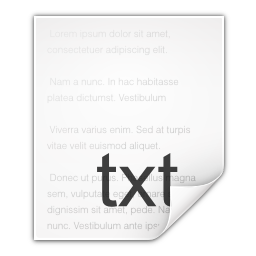
\includegraphics[width=0.05\textwidth]{tree/Mimetypes-text-plain-icon} Releases notes }.
.2 { 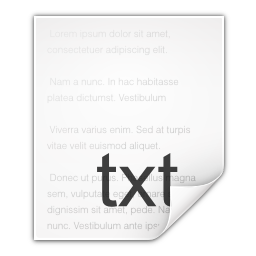
\includegraphics[width=0.05\textwidth]{tree/Mimetypes-text-plain-icon} TODO }.
.2 { 
\includegraphics[width=0.05\textwidth]{tree/Mimetypes-x-office-document-icon} LICENSE }.
.2 { 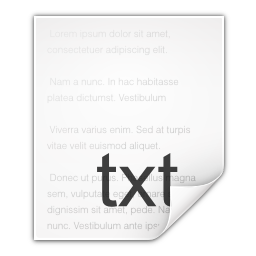
\includegraphics[width=0.05\textwidth]{tree/Mimetypes-text-plain-icon} CMakeLists.txt }.
.2 { 
\includegraphics[width=0.05\textwidth]{tree/Mimetypes-application-x-shellscript-icon} countLines.sh }.
.2 { 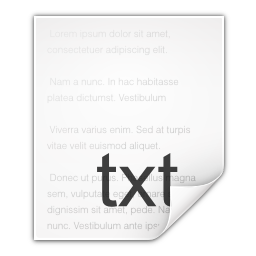
\includegraphics[width=0.05\textwidth]{tree/Mimetypes-text-plain-icon} Code styling }.
.2 { 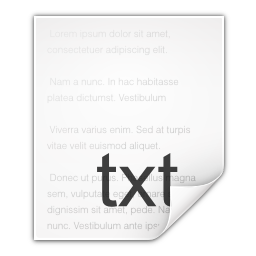
\includegraphics[width=0.05\textwidth]{tree/Mimetypes-text-plain-icon} config.h.cmake }.
.2 { 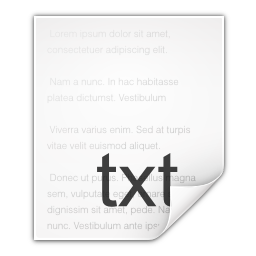
\includegraphics[width=0.05\textwidth]{tree/Mimetypes-text-plain-icon} README.md }.
.2 { 
\includegraphics[width=0.05\textwidth]{tree/Actions-document-open-folder-icon} doc }.
.3 { 
\includegraphics[width=0.05\textwidth]{tree/Mimetypes-application-pdf-icon} opencl-1-1-quick-reference-card.pdf }.
.3 { 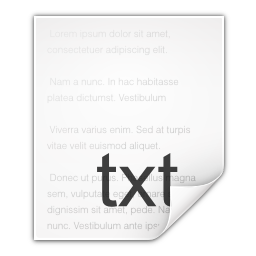
\includegraphics[width=0.05\textwidth]{tree/Mimetypes-text-plain-icon} CMakeLists.txt }.
.3 { 
\includegraphics[width=0.05\textwidth]{tree/Mimetypes-application-pdf-icon} Doxygen Quick Reference.pdf }.
.3 { 
\includegraphics[width=0.05\textwidth]{tree/Actions-document-open-folder-icon} cMake }.
.4 { 
\includegraphics[width=0.05\textwidth]{tree/Mimetypes-x-office-document-icon} Doxyfile.in }.
.3 { 
\includegraphics[width=0.05\textwidth]{tree/Actions-document-open-folder-icon} devManual }.
.4 { 
\includegraphics[width=0.05\textwidth]{tree/Mimetypes-application-pdf-icon} aquagpusph-devmanual.pdf }.
.4 { 
\includegraphics[width=0.05\textwidth]{tree/Mimetypes-x-office-document-icon} main.bbl }.
.4 { 
\includegraphics[width=0.05\textwidth]{tree/Mimetypes-text-x-bibtex-icon} directory\_tree.tex }.
.4 { 
\includegraphics[width=0.05\textwidth]{tree/Mimetypes-x-office-document-icon} main.aux }.
.4 { 
\includegraphics[width=0.05\textwidth]{tree/Mimetypes-x-office-document-icon} main.out }.
.4 { 
\includegraphics[width=0.05\textwidth]{tree/Mimetypes-text-x-bibtex-icon} structure.tex }.
.4 { 
\includegraphics[width=0.05\textwidth]{tree/Mimetypes-text-x-bibtex-icon} abstract.tex }.
.4 { 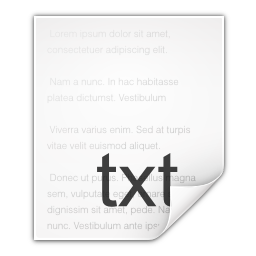
\includegraphics[width=0.05\textwidth]{tree/Mimetypes-text-plain-icon} main.log }.
.4 { 
\includegraphics[width=0.05\textwidth]{tree/Mimetypes-application-x-shellscript-icon} buildPDF.sh }.
.4 { 
\includegraphics[width=0.05\textwidth]{tree/Mimetypes-x-office-document-icon} main.blg }.
.4 { 
\includegraphics[width=0.05\textwidth]{tree/Mimetypes-x-office-document-icon} main.toc }.
.4 { 
\includegraphics[width=0.05\textwidth]{tree/Mimetypes-text-x-bibtex-icon} main.tex }.
.4 { 
\includegraphics[width=0.05\textwidth]{tree/Mimetypes-text-x-bibtex-icon} tree\_py.tex }.
.3 { 
\includegraphics[width=0.05\textwidth]{tree/Actions-document-open-folder-icon} userManual }.
.4 { 
\includegraphics[width=0.05\textwidth]{tree/Mimetypes-text-x-bibtex-icon} running.tex }.
.4 { 
\includegraphics[width=0.05\textwidth]{tree/Mimetypes-text-x-bibtex-icon} lateral\_water\_1x\_ghost.tex }.
.4 { 
\includegraphics[width=0.05\textwidth]{tree/Mimetypes-text-x-bibtex-icon} warningMsg.tex }.
.4 { 
\includegraphics[width=0.05\textwidth]{tree/Mimetypes-x-office-document-icon} main.bbl }.
.4 { 
\includegraphics[width=0.05\textwidth]{tree/Mimetypes-text-x-bibtex-icon} elasticbounce.tex }.
.4 { 
\includegraphics[width=0.05\textwidth]{tree/Mimetypes-text-x-bibtex-icon} errorMsg.tex }.
.4 { 
\includegraphics[width=0.05\textwidth]{tree/Mimetypes-text-x-bibtex-icon} directory\_tree.tex }.
.4 { 
\includegraphics[width=0.05\textwidth]{tree/Mimetypes-text-x-bibtex-icon} examples.tex }.
.4 { 
\includegraphics[width=0.05\textwidth]{tree/Mimetypes-text-x-bibtex-icon} asciiPartsInput.tex }.
.4 { 
\includegraphics[width=0.05\textwidth]{tree/Mimetypes-x-office-document-icon} main.aux }.
.4 { 
\includegraphics[width=0.05\textwidth]{tree/Mimetypes-text-x-bibtex-icon} motionTypes.tex }.
.4 { 
\includegraphics[width=0.05\textwidth]{tree/Mimetypes-text-x-bibtex-icon} paraview.tex }.
.4 { 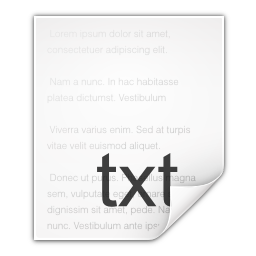
\includegraphics[width=0.05\textwidth]{tree/Mimetypes-text-plain-icon} texput.log }.
.4 { 
\includegraphics[width=0.05\textwidth]{tree/Mimetypes-text-x-bibtex-icon} sensors.tex }.
.4 { 
\includegraphics[width=0.05\textwidth]{tree/Mimetypes-text-x-bibtex-icon} DeLeffe.tex }.
.4 { 
\includegraphics[width=0.05\textwidth]{tree/Mimetypes-text-x-bibtex-icon} infoMsg.tex }.
.4 { 
\includegraphics[width=0.05\textwidth]{tree/Mimetypes-text-x-bibtex-icon} ghostparticles.tex }.
.4 { 
\includegraphics[width=0.05\textwidth]{tree/Mimetypes-x-office-document-icon} main.out }.
.4 { \includegraphics[width=0.05\textwidth]{tree/Mimetypes-text-x-bibtex-icon} partsInput.tex }.
.4 { \includegraphics[width=0.05\textwidth]{tree/Mimetypes-text-x-bibtex-icon} aquagpusph.tex }.
.4 { \includegraphics[width=0.05\textwidth]{tree/Mimetypes-text-x-bibtex-icon} abstract.tex }.
.4 { \includegraphics[width=0.05\textwidth]{tree/Mimetypes-text-plain-icon} main.log }.
.4 { \includegraphics[width=0.05\textwidth]{tree/Mimetypes-text-x-bibtex-icon} xmlPartsInput.tex }.
.4 { \includegraphics[width=0.05\textwidth]{tree/Mimetypes-text-x-bibtex-icon} lateral\_water\_1x\_deleffe.tex }.
.4 { \includegraphics[width=0.05\textwidth]{tree/Mimetypes-application-x-shellscript-icon} buildPDF.sh }.
.4 { \includegraphics[width=0.05\textwidth]{tree/Mimetypes-x-office-document-icon} bib.bib }.
.4 { \includegraphics[width=0.05\textwidth]{tree/Mimetypes-application-pdf-icon} aquagpusph-usermanual.pdf }.
.4 { \includegraphics[width=0.05\textwidth]{tree/Mimetypes-text-x-bibtex-icon} physics.tex }.
.4 { \includegraphics[width=0.05\textwidth]{tree/Mimetypes-x-office-document-icon} main.blg }.
.4 { \includegraphics[width=0.05\textwidth]{tree/Mimetypes-text-x-bibtex-icon} install.tex }.
.4 { \includegraphics[width=0.05\textwidth]{tree/Mimetypes-x-office-document-icon} main.toc }.
.4 { \includegraphics[width=0.05\textwidth]{tree/Mimetypes-text-x-bibtex-icon} fixparticles.tex }.
.4 { \includegraphics[width=0.05\textwidth]{tree/Mimetypes-text-x-bibtex-icon} outputFiles.tex }.
.4 { \includegraphics[width=0.05\textwidth]{tree/Mimetypes-text-x-bibtex-icon} main.tex }.
.4 { \includegraphics[width=0.05\textwidth]{tree/Mimetypes-text-x-bibtex-icon} gidPartsInput.tex }.
.4 { \includegraphics[width=0.05\textwidth]{tree/Mimetypes-text-x-bibtex-icon} tree\_py.tex }.
.4 { \includegraphics[width=0.05\textwidth]{tree/Mimetypes-text-x-bibtex-icon} xmlInput.tex }.
.4 { \includegraphics[width=0.05\textwidth]{tree/Mimetypes-text-x-bibtex-icon} motionControls.tex }.
.4 { \includegraphics[width=0.05\textwidth]{tree/Actions-document-open-folder-icon} images }.
.5 { \includegraphics[width=0.05\textwidth]{tree/Mimetypes-application-x-egon-icon} GhostParticlesCorner.svg }.
.5 { \includegraphics[width=0.05\textwidth]{tree/Mimetypes-application-x-egon-icon} FixedParticles.png }.
.5 { \includegraphics[width=0.05\textwidth]{tree/Mimetypes-application-x-egon-icon} DeLeffeCorner.svg }.
.5 { \includegraphics[width=0.05\textwidth]{tree/Mimetypes-application-x-egon-icon} GhostParticles.svg }.
.5 { \includegraphics[width=0.05\textwidth]{tree/Mimetypes-application-x-egon-icon} SPHInterpolation.png }.
.5 { \includegraphics[width=0.05\textwidth]{tree/Mimetypes-application-x-egon-icon} FixedParticles.svg }.
.5 { \includegraphics[width=0.05\textwidth]{tree/Mimetypes-application-x-egon-icon} ElasticBounce.svg }.
.5 { \includegraphics[width=0.05\textwidth]{tree/Mimetypes-application-x-egon-icon} GhostParticles.png }.
.5 { \includegraphics[width=0.05\textwidth]{tree/Mimetypes-application-x-egon-icon} LinkList.png }.
.5 { \includegraphics[width=0.05\textwidth]{tree/Mimetypes-application-x-egon-icon} ElasticBounce.png }.
.5 { \includegraphics[width=0.05\textwidth]{tree/Mimetypes-application-x-egon-icon} BC.png }.
.5 { \includegraphics[width=0.05\textwidth]{tree/Mimetypes-application-x-egon-icon} CoalescenceRead.png }.
.5 { \includegraphics[width=0.05\textwidth]{tree/Mimetypes-application-x-egon-icon} DeLeffe.svg }.
.5 { \includegraphics[width=0.05\textwidth]{tree/Mimetypes-application-x-egon-icon} DeLeffeCorner.png }.
.5 { \includegraphics[width=0.05\textwidth]{tree/Mimetypes-application-x-egon-icon} GhostParticlesCorner.png }.
.5 { \includegraphics[width=0.05\textwidth]{tree/Mimetypes-application-x-egon-icon} BC.svg }.
.5 { \includegraphics[width=0.05\textwidth]{tree/Mimetypes-application-x-egon-icon} SPHInterpolation.svg }.
.5 { \includegraphics[width=0.05\textwidth]{tree/Mimetypes-application-x-egon-icon} LinkList.svg }.
.5 { \includegraphics[width=0.05\textwidth]{tree/Mimetypes-application-x-egon-icon} DeLeffe.png }.
.5 { \includegraphics[width=0.05\textwidth]{tree/Mimetypes-application-x-egon-icon} CC\_88x31.png }.
.5 { \includegraphics[width=0.05\textwidth]{tree/Mimetypes-x-office-document-icon} Diagrams.odg }.
.5 { \includegraphics[width=0.05\textwidth]{tree/Mimetypes-application-x-egon-icon} GeneralDiagram.png }.
.5 { \includegraphics[width=0.05\textwidth]{tree/Actions-document-open-folder-icon} lateral\_water\_1x\_deleffe }.
.6 { \includegraphics[width=0.05\textwidth]{tree/Mimetypes-application-x-egon-icon} paraviewfluid3D.jpg }.
.6 { \includegraphics[width=0.05\textwidth]{tree/Mimetypes-application-x-egon-icon} animation\_freeslip.jpg }.
.6 { \includegraphics[width=0.05\textwidth]{tree/Mimetypes-application-x-egon-icon} particles.png }.
.6 { \includegraphics[width=0.05\textwidth]{tree/Mimetypes-application-x-egon-icon} animation\_noslip.jpg }.
.6 { \includegraphics[width=0.05\textwidth]{tree/Mimetypes-application-pdf-icon} press.pdf }.
.6 { \includegraphics[width=0.05\textwidth]{tree/Mimetypes-application-x-egon-icon} paraviewcolormap.jpg }.
.6 { \includegraphics[width=0.05\textwidth]{tree/Mimetypes-application-x-egon-icon} paraviewfilter.jpg }.
.6 { \includegraphics[width=0.05\textwidth]{tree/Mimetypes-application-x-egon-icon} tank.png }.
.6 { \includegraphics[width=0.05\textwidth]{tree/Mimetypes-application-x-egon-icon} sensors\_noslip.png }.
.6 { \includegraphics[width=0.05\textwidth]{tree/Mimetypes-application-x-egon-icon} particles.svg }.
.6 { \includegraphics[width=0.05\textwidth]{tree/Mimetypes-application-x-egon-icon} paraviewfilteroptions.jpg }.
.6 { \includegraphics[width=0.05\textwidth]{tree/Mimetypes-application-x-egon-icon} paraviewsolid3D.jpg }.
.6 { \includegraphics[width=0.05\textwidth]{tree/Mimetypes-application-x-egon-icon} sensors\_freeslip.png }.
.6 { \includegraphics[width=0.05\textwidth]{tree/Mimetypes-application-x-egon-icon} paraviewsolidfilter.jpg }.
.6 { \includegraphics[width=0.05\textwidth]{tree/Mimetypes-x-office-document-icon} lateral\_water\_1x.gnuplot }.
.5 { \includegraphics[width=0.05\textwidth]{tree/Actions-document-open-folder-icon} wendland }.
.6 { \includegraphics[width=0.05\textwidth]{tree/Mimetypes-application-pdf-icon} wendland2D.pdf }.
.6 { \includegraphics[width=0.05\textwidth]{tree/Mimetypes-text-x-python-icon} wendland2D.py }.
.5 { \includegraphics[width=0.05\textwidth]{tree/Actions-document-open-folder-icon} tree }.
.6 { \includegraphics[width=0.05\textwidth]{tree/Mimetypes-application-x-egon-icon} Mimetypes-application-x-shellscript-icon.png }.
.6 { \includegraphics[width=0.05\textwidth]{tree/Mimetypes-application-x-egon-icon} Mimetypes-text-x-bibtex-icon.png }.
.6 { \includegraphics[width=0.05\textwidth]{tree/Mimetypes-application-x-egon-icon} Mimetypes-application-vnd-oasis-opendocument-spreadsheet-icon.png }.
.6 { \includegraphics[width=0.05\textwidth]{tree/Mimetypes-application-x-egon-icon} Mimetypes-application-xml-icon.png }.
.6 { \includegraphics[width=0.05\textwidth]{tree/Mimetypes-application-x-egon-icon} Mimetypes-application-x-egon-icon.png }.
.6 { \includegraphics[width=0.05\textwidth]{tree/Mimetypes-application-x-egon-icon} Mimetypes-application-x-archive-icon.png }.
.6 { \includegraphics[width=0.05\textwidth]{tree/Mimetypes-application-x-egon-icon} Actions-edit-select-all-icon.png }.
.6 { \includegraphics[width=0.05\textwidth]{tree/Mimetypes-application-x-egon-icon} Mimetypes-application-rtf-icon.png }.
.6 { \includegraphics[width=0.05\textwidth]{tree/Mimetypes-application-x-egon-icon} Mimetypes-text-x-c-plus-plus-src-icon.png }.
.6 { \includegraphics[width=0.05\textwidth]{tree/Mimetypes-text-x-python-icon} tree.py }.
.6 { \includegraphics[width=0.05\textwidth]{tree/Mimetypes-application-x-egon-icon} Mimetypes-text-plain-icon.png }.
.6 { \includegraphics[width=0.05\textwidth]{tree/Mimetypes-application-x-egon-icon} Mimetypes-text-x-csrc-icon.png }.
.6 { \includegraphics[width=0.05\textwidth]{tree/Mimetypes-application-x-egon-icon} Mimetypes-text-x-python-icon.png }.
.6 { \includegraphics[width=0.05\textwidth]{tree/Mimetypes-application-x-egon-icon} Mimetypes-application-x-applix-word-icon.png }.
.6 { \includegraphics[width=0.05\textwidth]{tree/Mimetypes-application-x-egon-icon} Mimetypes-application-x-desktop-icon.png }.
.6 { \includegraphics[width=0.05\textwidth]{tree/Mimetypes-application-x-egon-icon} Mimetypes-x-office-document-icon.png }.
.6 { \includegraphics[width=0.05\textwidth]{tree/Mimetypes-application-x-egon-icon} Mimetypes-application-vnd-oasis-opendocument-graphics-icon.png }.
.6 { \includegraphics[width=0.05\textwidth]{tree/Mimetypes-application-x-egon-icon} Mimetypes-application-vnd-stardivision-draw-icon.png }.
.6 { \includegraphics[width=0.05\textwidth]{tree/Mimetypes-application-x-egon-icon} Mimetypes-application-pdf-icon.png }.
.6 { \includegraphics[width=0.05\textwidth]{tree/Mimetypes-application-x-egon-icon} Mimetypes-application-octet-stream-icon.png }.
.6 { \includegraphics[width=0.05\textwidth]{tree/Mimetypes-application-x-egon-icon} Mimetypes-text-x-chdr-icon.png }.
.6 { \includegraphics[width=0.05\textwidth]{tree/Mimetypes-application-x-egon-icon} Actions-document-open-folder-icon.png }.
.5 { \includegraphics[width=0.05\textwidth]{tree/Actions-document-open-folder-icon} lateral\_water\_1x\_ghost }.
.6 { \includegraphics[width=0.05\textwidth]{tree/Mimetypes-application-x-egon-icon} animation\_freeslip.jpg }.
.6 { \includegraphics[width=0.05\textwidth]{tree/Mimetypes-application-x-egon-icon} sensors\_noslip.png }.
.6 { \includegraphics[width=0.05\textwidth]{tree/Mimetypes-application-x-egon-icon} sensors\_freeslip.png }.
.2 { \includegraphics[width=0.05\textwidth]{tree/Actions-document-open-folder-icon} tools }.
.3 { \includegraphics[width=0.05\textwidth]{tree/Mimetypes-text-x-python-icon} setup.py }.
.3 { \includegraphics[width=0.05\textwidth]{tree/Mimetypes-text-plain-icon} CMakeLists.txt }.
.3 { \includegraphics[width=0.05\textwidth]{tree/Actions-document-open-folder-icon} aquagpusph\_postprocessing }.
.4 { \includegraphics[width=0.05\textwidth]{tree/Mimetypes-x-office-document-icon} vtk-freesurface }.
.4 { \includegraphics[width=0.05\textwidth]{tree/Mimetypes-x-office-document-icon} pvd-locale }.
.3 { \includegraphics[width=0.05\textwidth]{tree/Actions-document-open-folder-icon} aquagpusph\_preprocessing }.
.4 { \includegraphics[width=0.05\textwidth]{tree/Mimetypes-x-office-document-icon} AQUAgpusph-loadGiD }.
.4 { \includegraphics[width=0.05\textwidth]{tree/Mimetypes-x-office-document-icon} AQUAgpusph-loadAbaqus }.
.4 { \includegraphics[width=0.05\textwidth]{tree/Mimetypes-text-x-python-icon} \_\_init\_\_.py }.
.4 { \includegraphics[width=0.05\textwidth]{tree/Actions-document-open-folder-icon} generator }.
.5 { \includegraphics[width=0.05\textwidth]{tree/Mimetypes-text-x-python-icon} fluid.py }.
.5 { \includegraphics[width=0.05\textwidth]{tree/Mimetypes-text-x-python-icon} vec.py }.
.5 { \includegraphics[width=0.05\textwidth]{tree/Mimetypes-text-x-python-icon} solid.py }.
.5 { \includegraphics[width=0.05\textwidth]{tree/Mimetypes-text-x-python-icon} \_\_init\_\_.py }.
.4 { \includegraphics[width=0.05\textwidth]{tree/Actions-document-open-folder-icon} mesh\_loader }.
.5 { \includegraphics[width=0.05\textwidth]{tree/Mimetypes-text-x-python-icon} Abaqus.py }.
.5 { \includegraphics[width=0.05\textwidth]{tree/Mimetypes-text-x-python-icon} GiD.py }.
.5 { \includegraphics[width=0.05\textwidth]{tree/Mimetypes-text-x-python-icon} \_\_init\_\_.py }.
.2 { \includegraphics[width=0.05\textwidth]{tree/Actions-document-open-folder-icon} examples }.
.3 { \includegraphics[width=0.05\textwidth]{tree/Mimetypes-text-plain-icon} CMakeLists.txt }.
.3 { \includegraphics[width=0.05\textwidth]{tree/Actions-document-open-folder-icon} LateralWater\_1x\_Ghost }.
.4 { \includegraphics[width=0.05\textwidth]{tree/Mimetypes-text-x-python-icon} Create.py }.
.4 { \includegraphics[width=0.05\textwidth]{tree/Actions-document-open-folder-icon} doc }.
.5 { \includegraphics[width=0.05\textwidth]{tree/Mimetypes-text-x-python-icon} plot.py }.
.5 { \includegraphics[width=0.05\textwidth]{tree/Mimetypes-application-pdf-icon} SOUTOIGLESIAS\_BOTIA\_SPHERIC\_TESTCASE\_10.pdf }.
.5 { \includegraphics[width=0.05\textwidth]{tree/Mimetypes-text-plain-icon} lateral\_water\_1x.txt }.
.4 { \includegraphics[width=0.05\textwidth]{tree/Actions-document-open-folder-icon} Move }.
.5 { \includegraphics[width=0.05\textwidth]{tree/Mimetypes-x-office-document-icon} 6DOFresources.ods }.
.5 { \includegraphics[width=0.05\textwidth]{tree/Mimetypes-text-plain-icon} 6DOF.dat }.
.3 { \includegraphics[width=0.05\textwidth]{tree/Actions-document-open-folder-icon} cMake }.
.4 { \includegraphics[width=0.05\textwidth]{tree/Actions-document-open-folder-icon} LateralWater\_1x\_Ghost }.
.5 { \includegraphics[width=0.05\textwidth]{tree/Mimetypes-application-xml-icon} Fluids.xml }.
.5 { \includegraphics[width=0.05\textwidth]{tree/Mimetypes-application-xml-icon} GhostParticles.xml }.
.5 { \includegraphics[width=0.05\textwidth]{tree/Mimetypes-application-xml-icon} Time.xml }.
.5 { \includegraphics[width=0.05\textwidth]{tree/Mimetypes-application-xml-icon} Sensors.xml }.
.5 { \includegraphics[width=0.05\textwidth]{tree/Mimetypes-application-x-shellscript-icon} run.sh }.
.5 { \includegraphics[width=0.05\textwidth]{tree/Mimetypes-application-xml-icon} Movements.xml }.
.5 { \includegraphics[width=0.05\textwidth]{tree/Mimetypes-application-xml-icon} Settings.xml }.
.5 { \includegraphics[width=0.05\textwidth]{tree/Mimetypes-application-xml-icon} SPH.xml }.
.5 { \includegraphics[width=0.05\textwidth]{tree/Mimetypes-application-xml-icon} Main.xml }.
.5 { \includegraphics[width=0.05\textwidth]{tree/Actions-document-open-folder-icon} Move }.
.6 { \includegraphics[width=0.05\textwidth]{tree/Mimetypes-application-xml-icon} 6DOF.xml }.
.4 { \includegraphics[width=0.05\textwidth]{tree/Actions-document-open-folder-icon} LateralWater\_1x\_Fix }.
.5 { \includegraphics[width=0.05\textwidth]{tree/Mimetypes-application-xml-icon} Fluids.xml }.
.5 { \includegraphics[width=0.05\textwidth]{tree/Mimetypes-application-xml-icon} Time.xml }.
.5 { \includegraphics[width=0.05\textwidth]{tree/Mimetypes-application-xml-icon} Sensors.xml }.
.5 { \includegraphics[width=0.05\textwidth]{tree/Mimetypes-application-x-shellscript-icon} run.sh }.
.5 { \includegraphics[width=0.05\textwidth]{tree/Mimetypes-application-xml-icon} Movements.xml }.
.5 { \includegraphics[width=0.05\textwidth]{tree/Mimetypes-application-xml-icon} Settings.xml }.
.5 { \includegraphics[width=0.05\textwidth]{tree/Mimetypes-application-xml-icon} SPH.xml }.
.5 { \includegraphics[width=0.05\textwidth]{tree/Mimetypes-application-xml-icon} Main.xml }.
.5 { \includegraphics[width=0.05\textwidth]{tree/Actions-document-open-folder-icon} Move }.
.6 { \includegraphics[width=0.05\textwidth]{tree/Mimetypes-application-xml-icon} 6DOF.xml }.
.4 { \includegraphics[width=0.05\textwidth]{tree/Actions-document-open-folder-icon} perezrojas\_etal\_stab\_2012 }.
.5 { \includegraphics[width=0.05\textwidth]{tree/Mimetypes-application-xml-icon} Fluids.xml }.
.5 { \includegraphics[width=0.05\textwidth]{tree/Mimetypes-application-xml-icon} Time.xml }.
.5 { \includegraphics[width=0.05\textwidth]{tree/Mimetypes-application-x-shellscript-icon} run.sh }.
.5 { \includegraphics[width=0.05\textwidth]{tree/Mimetypes-application-xml-icon} Movements.xml }.
.5 { \includegraphics[width=0.05\textwidth]{tree/Mimetypes-application-xml-icon} Settings.xml }.
.5 { \includegraphics[width=0.05\textwidth]{tree/Mimetypes-application-xml-icon} SPH.xml }.
.5 { \includegraphics[width=0.05\textwidth]{tree/Mimetypes-application-xml-icon} Main.xml }.
.5 { \includegraphics[width=0.05\textwidth]{tree/Actions-document-open-folder-icon} Move }.
.6 { \includegraphics[width=0.05\textwidth]{tree/Mimetypes-text-x-python-icon} move.py }.
.6 { \includegraphics[width=0.05\textwidth]{tree/Mimetypes-application-xml-icon} 6DOF.xml }.
.4 { \includegraphics[width=0.05\textwidth]{tree/Actions-document-open-folder-icon} lobovsky\_etal\_jfs\_2014 }.
.5 { \includegraphics[width=0.05\textwidth]{tree/Mimetypes-application-xml-icon} Fluids.xml }.
.5 { \includegraphics[width=0.05\textwidth]{tree/Mimetypes-application-xml-icon} Time.xml }.
.5 { \includegraphics[width=0.05\textwidth]{tree/Mimetypes-application-xml-icon} Sensors.xml }.
.5 { \includegraphics[width=0.05\textwidth]{tree/Mimetypes-application-x-shellscript-icon} run.sh }.
.5 { \includegraphics[width=0.05\textwidth]{tree/Mimetypes-application-xml-icon} Settings.xml }.
.5 { \includegraphics[width=0.05\textwidth]{tree/Mimetypes-application-xml-icon} SPH.xml }.
.5 { \includegraphics[width=0.05\textwidth]{tree/Mimetypes-application-xml-icon} Main.xml }.
.4 { \includegraphics[width=0.05\textwidth]{tree/Actions-document-open-folder-icon} LateralWater\_1x\_DeLeffe }.
.5 { \includegraphics[width=0.05\textwidth]{tree/Mimetypes-application-xml-icon} Fluids.xml }.
.5 { \includegraphics[width=0.05\textwidth]{tree/Mimetypes-application-xml-icon} Time.xml }.
.5 { \includegraphics[width=0.05\textwidth]{tree/Mimetypes-application-xml-icon} Sensors.xml }.
.5 { \includegraphics[width=0.05\textwidth]{tree/Mimetypes-application-x-shellscript-icon} run.sh }.
.5 { \includegraphics[width=0.05\textwidth]{tree/Mimetypes-application-xml-icon} Movements.xml }.
.5 { \includegraphics[width=0.05\textwidth]{tree/Mimetypes-application-xml-icon} Settings.xml }.
.5 { \includegraphics[width=0.05\textwidth]{tree/Mimetypes-application-xml-icon} SPH.xml }.
.5 { \includegraphics[width=0.05\textwidth]{tree/Mimetypes-application-xml-icon} Main.xml }.
.5 { \includegraphics[width=0.05\textwidth]{tree/Actions-document-open-folder-icon} Move }.
.6 { \includegraphics[width=0.05\textwidth]{tree/Mimetypes-application-xml-icon} 6DOF.xml }.
.3 { \includegraphics[width=0.05\textwidth]{tree/Actions-document-open-folder-icon} LateralWater\_1x\_Fix }.
.4 { \includegraphics[width=0.05\textwidth]{tree/Mimetypes-text-x-python-icon} Create.py }.
.4 { \includegraphics[width=0.05\textwidth]{tree/Actions-document-open-folder-icon} doc }.
.5 { \includegraphics[width=0.05\textwidth]{tree/Mimetypes-text-x-python-icon} plot.py }.
.5 { \includegraphics[width=0.05\textwidth]{tree/Mimetypes-application-pdf-icon} SOUTOIGLESIAS\_BOTIA\_SPHERIC\_TESTCASE\_10.pdf }.
.5 { \includegraphics[width=0.05\textwidth]{tree/Mimetypes-text-plain-icon} lateral\_water\_1x.txt }.
.4 { \includegraphics[width=0.05\textwidth]{tree/Actions-document-open-folder-icon} Move }.
.5 { \includegraphics[width=0.05\textwidth]{tree/Mimetypes-x-office-document-icon} 6DOFresources.ods }.
.5 { \includegraphics[width=0.05\textwidth]{tree/Mimetypes-text-plain-icon} 6DOF.dat }.
.3 { \includegraphics[width=0.05\textwidth]{tree/Actions-document-open-folder-icon} perezrojas\_etal\_stab\_2012 }.
.4 { \includegraphics[width=0.05\textwidth]{tree/Mimetypes-text-x-python-icon} Create.py }.
.4 { \includegraphics[width=0.05\textwidth]{tree/Actions-document-open-folder-icon} doc }.
.5 { \includegraphics[width=0.05\textwidth]{tree/Mimetypes-text-x-python-icon} plot.py }.
.5 { \includegraphics[width=0.05\textwidth]{tree/Mimetypes-application-pdf-icon} SOUTOIGLESIAS\_BOTIA\_SPHERIC\_TESTCASE9\_TLD.pdf }.
.4 { \includegraphics[width=0.05\textwidth]{tree/Actions-document-open-folder-icon} Move }.
.5 { \includegraphics[width=0.05\textwidth]{tree/Mimetypes-text-plain-icon} T\_1-94\_A100mm\_water.dat }.
.3 { \includegraphics[width=0.05\textwidth]{tree/Actions-document-open-folder-icon} lobovsky\_etal\_jfs\_2014 }.
.4 { \includegraphics[width=0.05\textwidth]{tree/Mimetypes-text-x-python-icon} Create.py }.
.4 { \includegraphics[width=0.05\textwidth]{tree/Actions-document-open-folder-icon} doc }.
.5 { \includegraphics[width=0.05\textwidth]{tree/Mimetypes-text-plain-icon} Fig30\_filtered\_5.dat }.
.5 { \includegraphics[width=0.05\textwidth]{tree/Mimetypes-text-plain-icon} Fig20\_filtered\_2.dat }.
.5 { \includegraphics[width=0.05\textwidth]{tree/Mimetypes-text-plain-icon} Fig12\_02\_ETSIN\_Front\_Hu\_Koshizuka\_3.dat }.
.5 { \includegraphics[width=0.05\textwidth]{tree/Mimetypes-text-plain-icon} Fig29\_filtered\_3.dat }.
.5 { \includegraphics[width=0.05\textwidth]{tree/Mimetypes-text-plain-icon} Fig31\_filtered\_1.dat }.
.5 { \includegraphics[width=0.05\textwidth]{tree/Mimetypes-text-plain-icon} Fig12\_01\_ETSIN\_Front\_Dressler\_Martin\_4.dat }.
.5 { \includegraphics[width=0.05\textwidth]{tree/Mimetypes-text-x-python-icon} sensor3.py }.
.5 { \includegraphics[width=0.05\textwidth]{tree/Mimetypes-text-plain-icon} Fig12\_01\_ETSIN\_Front\_Dressler\_Martin\_7.dat }.
.5 { \includegraphics[width=0.05\textwidth]{tree/Mimetypes-text-plain-icon} Fig12\_01\_ETSIN\_Front\_Dressler\_Martin\_6.dat }.
.5 { \includegraphics[width=0.05\textwidth]{tree/Mimetypes-text-plain-icon} Fig30\_filtered\_2.dat }.
.5 { \includegraphics[width=0.05\textwidth]{tree/Mimetypes-text-plain-icon} Fig12\_01\_ETSIN\_Front\_Dressler\_Martin\_3.dat }.
.5 { \includegraphics[width=0.05\textwidth]{tree/Mimetypes-text-plain-icon} Fig29\_filtered\_2.dat }.
.5 { \includegraphics[width=0.05\textwidth]{tree/Mimetypes-text-plain-icon} Fig31\_filtered\_4.dat }.
.5 { \includegraphics[width=0.05\textwidth]{tree/Mimetypes-text-plain-icon} Fig12\_01\_ETSIN\_Front\_Dressler\_Martin\_5.dat }.
.5 { \includegraphics[width=0.05\textwidth]{tree/Mimetypes-text-plain-icon} Fig31\_filtered\_2.dat }.
.5 { \includegraphics[width=0.05\textwidth]{tree/Mimetypes-text-plain-icon} Fig30\_filtered\_4.dat }.
.5 { \includegraphics[width=0.05\textwidth]{tree/Mimetypes-text-x-python-icon} performance.py }.
.5 { \includegraphics[width=0.05\textwidth]{tree/Mimetypes-text-plain-icon} Fig12\_01\_ETSIN\_Front\_Dressler\_Martin\_2.dat }.
.5 { \includegraphics[width=0.05\textwidth]{tree/Mimetypes-text-plain-icon} Fig29\_filtered\_4.dat }.
.5 { \includegraphics[width=0.05\textwidth]{tree/Mimetypes-text-plain-icon} Fig12\_02\_ETSIN\_Front\_Hu\_Koshizuka\_5.dat }.
.5 { \includegraphics[width=0.05\textwidth]{tree/Mimetypes-text-x-python-icon} sensor2.py }.
.5 { \includegraphics[width=0.05\textwidth]{tree/Mimetypes-text-x-python-icon} sensor1.py }.
.5 { \includegraphics[width=0.05\textwidth]{tree/Mimetypes-text-x-python-icon} sensor4.py }.
.5 { \includegraphics[width=0.05\textwidth]{tree/Mimetypes-text-plain-icon} Fig30\_filtered\_1.dat }.
.5 { \includegraphics[width=0.05\textwidth]{tree/Mimetypes-text-plain-icon} Fig29\_filtered\_1.dat }.
.5 { \includegraphics[width=0.05\textwidth]{tree/Mimetypes-text-plain-icon} Fig12\_02\_ETSIN\_Front\_Hu\_Koshizuka\_4.dat }.
.5 { \includegraphics[width=0.05\textwidth]{tree/Mimetypes-text-x-python-icon} sensors.py }.
.5 { \includegraphics[width=0.05\textwidth]{tree/Mimetypes-text-plain-icon} Fig20\_filtered\_3.dat }.
.5 { \includegraphics[width=0.05\textwidth]{tree/Mimetypes-text-plain-icon} Fig30\_filtered\_3.dat }.
.5 { \includegraphics[width=0.05\textwidth]{tree/Mimetypes-text-plain-icon} Fig20\_filtered\_1.dat }.
.5 { \includegraphics[width=0.05\textwidth]{tree/Mimetypes-text-plain-icon} Fig31\_filtered\_3.dat }.
.3 { \includegraphics[width=0.05\textwidth]{tree/Actions-document-open-folder-icon} LateralWater\_1x\_DeLeffe }.
.4 { \includegraphics[width=0.05\textwidth]{tree/Mimetypes-text-x-python-icon} Create.py }.
.4 { \includegraphics[width=0.05\textwidth]{tree/Actions-document-open-folder-icon} doc }.
.5 { \includegraphics[width=0.05\textwidth]{tree/Mimetypes-text-x-python-icon} plot.py }.
.5 { \includegraphics[width=0.05\textwidth]{tree/Mimetypes-application-pdf-icon} SOUTOIGLESIAS\_BOTIA\_SPHERIC\_TESTCASE\_10.pdf }.
.5 { \includegraphics[width=0.05\textwidth]{tree/Mimetypes-text-plain-icon} lateral\_water\_1x.txt }.
.4 { \includegraphics[width=0.05\textwidth]{tree/Actions-document-open-folder-icon} Move }.
.5 { \includegraphics[width=0.05\textwidth]{tree/Mimetypes-x-office-document-icon} 6DOFresources.ods }.
.5 { \includegraphics[width=0.05\textwidth]{tree/Mimetypes-text-plain-icon} 6DOF.dat }.
.2 { \includegraphics[width=0.05\textwidth]{tree/Actions-document-open-folder-icon} cMake }.
.3 { \includegraphics[width=0.05\textwidth]{tree/Mimetypes-text-plain-icon} FindOpenCL.cmake }.
.3 { \includegraphics[width=0.05\textwidth]{tree/Mimetypes-text-plain-icon} Findhdf5.cmake }.
.3 { \includegraphics[width=0.05\textwidth]{tree/Mimetypes-text-plain-icon} FindCurses.cmake }.
.3 { \includegraphics[width=0.05\textwidth]{tree/Mimetypes-text-plain-icon} FindXerces.cmake }.
.3 { \includegraphics[width=0.05\textwidth]{tree/Mimetypes-text-plain-icon} ConfigureChecks.cmake }.
.3 { \includegraphics[width=0.05\textwidth]{tree/Mimetypes-text-plain-icon} FindH5Part.cmake }.
.3 { \includegraphics[width=0.05\textwidth]{tree/Mimetypes-text-plain-icon} FindEigen3.cmake }.
.3 { \includegraphics[width=0.05\textwidth]{tree/Mimetypes-text-plain-icon} Findmatheval.cmake }.
.2 { \includegraphics[width=0.05\textwidth]{tree/Actions-document-open-folder-icon} include }.
.3 { \includegraphics[width=0.05\textwidth]{tree/Mimetypes-text-plain-icon} CMakeLists.txt }.
.3 { \includegraphics[width=0.05\textwidth]{tree/Mimetypes-text-x-chdr-icon} ArgumentsManager.h }.
.3 { \includegraphics[width=0.05\textwidth]{tree/Mimetypes-text-x-chdr-icon} sphPrerequisites.h }.
.3 { \includegraphics[width=0.05\textwidth]{tree/Mimetypes-text-x-chdr-icon} Singleton.h }.
.3 { \includegraphics[width=0.05\textwidth]{tree/Mimetypes-text-x-chdr-icon} ScreenManager.h }.
.3 { \includegraphics[width=0.05\textwidth]{tree/Mimetypes-text-x-chdr-icon} AuxiliarMethods.h }.
.3 { \includegraphics[width=0.05\textwidth]{tree/Mimetypes-text-x-chdr-icon} ProblemSetup.h }.
.3 { \includegraphics[width=0.05\textwidth]{tree/Mimetypes-text-x-chdr-icon} TimeManager.h }.
.3 { \includegraphics[width=0.05\textwidth]{tree/Mimetypes-text-x-chdr-icon} Fluid.h }.
.3 { \includegraphics[width=0.05\textwidth]{tree/Mimetypes-text-x-chdr-icon} CalcServer.h }.
.3 { \includegraphics[width=0.05\textwidth]{tree/Mimetypes-text-x-chdr-icon} FileManager.h }.
.3 { \includegraphics[width=0.05\textwidth]{tree/Actions-document-open-folder-icon} Tokenizer }.
.4 { \includegraphics[width=0.05\textwidth]{tree/Mimetypes-text-x-chdr-icon} Tokenizer.h }.
.3 { \includegraphics[width=0.05\textwidth]{tree/Actions-document-open-folder-icon} CalcServer }.
.4 { \includegraphics[width=0.05\textwidth]{tree/Mimetypes-text-x-chdr-icon} Torque.h }.
.4 { \includegraphics[width=0.05\textwidth]{tree/Mimetypes-text-x-chdr-icon} RadixSort.h }.
.4 { \includegraphics[width=0.05\textwidth]{tree/Mimetypes-text-x-chdr-icon} Domain.h }.
.4 { \includegraphics[width=0.05\textwidth]{tree/Mimetypes-text-x-chdr-icon} Sensors.h }.
.4 { \includegraphics[width=0.05\textwidth]{tree/Mimetypes-text-x-chdr-icon} Bounds.h }.
.4 { \includegraphics[width=0.05\textwidth]{tree/Mimetypes-text-x-chdr-icon} Corrector.h }.
.4 { \includegraphics[width=0.05\textwidth]{tree/Mimetypes-text-x-chdr-icon} LinkList.h }.
.4 { \includegraphics[width=0.05\textwidth]{tree/Mimetypes-text-x-chdr-icon} Permutate.h }.
.4 { \includegraphics[width=0.05\textwidth]{tree/Mimetypes-text-x-chdr-icon} Grid.h }.
.4 { \includegraphics[width=0.05\textwidth]{tree/Mimetypes-text-x-chdr-icon} TimeStep.h }.
.4 { \includegraphics[width=0.05\textwidth]{tree/Mimetypes-text-x-chdr-icon} Rates.h }.
.4 { \includegraphics[width=0.05\textwidth]{tree/Mimetypes-text-x-chdr-icon} DensityInterpolation.h }.
.4 { \includegraphics[width=0.05\textwidth]{tree/Mimetypes-text-x-chdr-icon} Energy.h }.
.4 { \includegraphics[width=0.05\textwidth]{tree/Mimetypes-text-x-chdr-icon} Reduction.h }.
.4 { \includegraphics[width=0.05\textwidth]{tree/Mimetypes-text-x-chdr-icon} Kernel.h }.
.4 { \includegraphics[width=0.05\textwidth]{tree/Mimetypes-text-x-chdr-icon} Shepard.h }.
.4 { \includegraphics[width=0.05\textwidth]{tree/Mimetypes-text-x-chdr-icon} Predictor.h }.
.4 { \includegraphics[width=0.05\textwidth]{tree/Actions-document-open-folder-icon} Movements }.
.5 { \includegraphics[width=0.05\textwidth]{tree/Mimetypes-text-x-chdr-icon} Quaternion.h }.
.5 { \includegraphics[width=0.05\textwidth]{tree/Mimetypes-text-x-chdr-icon} ScriptQuaternion.h }.
.5 { \includegraphics[width=0.05\textwidth]{tree/Mimetypes-text-x-chdr-icon} C1Quaternion.h }.
.5 { \includegraphics[width=0.05\textwidth]{tree/Mimetypes-text-x-chdr-icon} Movement.h }.
.5 { \includegraphics[width=0.05\textwidth]{tree/Mimetypes-text-x-chdr-icon} LinearInterpolation.h }.
.5 { \includegraphics[width=0.05\textwidth]{tree/Mimetypes-text-x-chdr-icon} C1Interpolation.h }.
.5 { \includegraphics[width=0.05\textwidth]{tree/Mimetypes-text-x-chdr-icon} LIQuaternion.h }.
.4 { \includegraphics[width=0.05\textwidth]{tree/Actions-document-open-folder-icon} Portal }.
.5 { \includegraphics[width=0.05\textwidth]{tree/Mimetypes-text-x-chdr-icon} Portal.h }.
.4 { \includegraphics[width=0.05\textwidth]{tree/Actions-document-open-folder-icon} Boundary }.
.5 { \includegraphics[width=0.05\textwidth]{tree/Mimetypes-text-x-chdr-icon} ElasticBounce.h }.
.5 { \includegraphics[width=0.05\textwidth]{tree/Mimetypes-text-x-chdr-icon} GhostParticles.h }.
.5 { \includegraphics[width=0.05\textwidth]{tree/Mimetypes-text-x-chdr-icon} DeLeffe.h }.
.3 { \includegraphics[width=0.05\textwidth]{tree/Actions-document-open-folder-icon} InputOutput }.
.4 { \includegraphics[width=0.05\textwidth]{tree/Mimetypes-text-x-chdr-icon} Log.h }.
.4 { \includegraphics[width=0.05\textwidth]{tree/Mimetypes-text-x-chdr-icon} ASCII.h }.
.4 { \includegraphics[width=0.05\textwidth]{tree/Mimetypes-text-x-chdr-icon} Report.h }.
.4 { \includegraphics[width=0.05\textwidth]{tree/Mimetypes-text-x-chdr-icon} InputOutput.h }.
.4 { \includegraphics[width=0.05\textwidth]{tree/Mimetypes-text-x-chdr-icon} State.h }.
.4 { \includegraphics[width=0.05\textwidth]{tree/Mimetypes-text-x-chdr-icon} Bounds.h }.
.4 { \includegraphics[width=0.05\textwidth]{tree/Mimetypes-text-x-chdr-icon} VTK.h }.
.4 { \includegraphics[width=0.05\textwidth]{tree/Mimetypes-text-x-chdr-icon} Energy.h }.
.4 { \includegraphics[width=0.05\textwidth]{tree/Mimetypes-text-x-chdr-icon} Particles.h }.
.2 { \includegraphics[width=0.05\textwidth]{tree/Actions-document-open-folder-icon} resources }.
.3 { \includegraphics[width=0.05\textwidth]{tree/Mimetypes-x-office-document-icon} OpenCLMain.xml.in }.
.3 { \includegraphics[width=0.05\textwidth]{tree/Mimetypes-text-plain-icon} CMakeLists.txt }.
.3 { \includegraphics[width=0.05\textwidth]{tree/Actions-document-open-folder-icon} OpenCL }.
.4 { \includegraphics[width=0.05\textwidth]{tree/Mimetypes-text-x-csrc-icon} LinkList.cl }.
.4 { \includegraphics[width=0.05\textwidth]{tree/Mimetypes-text-x-csrc-icon} Corrector.cl }.
.4 { \includegraphics[width=0.05\textwidth]{tree/Mimetypes-text-x-chdr-icon} RatesSensors.hcl }.
.4 { \includegraphics[width=0.05\textwidth]{tree/Mimetypes-text-x-csrc-icon} Shepard.cl }.
.4 { \includegraphics[width=0.05\textwidth]{tree/Mimetypes-text-x-csrc-icon} Rates.cl }.
.4 { \includegraphics[width=0.05\textwidth]{tree/Mimetypes-text-x-chdr-icon} RatesBounds.hcl }.
.4 { \includegraphics[width=0.05\textwidth]{tree/Mimetypes-text-x-csrc-icon} Energy.cl }.
.4 { \includegraphics[width=0.05\textwidth]{tree/Mimetypes-text-x-csrc-icon} Permutate.cl }.
.4 { \includegraphics[width=0.05\textwidth]{tree/Mimetypes-text-x-csrc-icon} DensInt.cl }.
.4 { \includegraphics[width=0.05\textwidth]{tree/Mimetypes-text-x-csrc-icon} RadixSort.cl }.
.4 { \includegraphics[width=0.05\textwidth]{tree/Mimetypes-text-x-csrc-icon} Torque.cl }.
.4 { \includegraphics[width=0.05\textwidth]{tree/Mimetypes-text-x-csrc-icon} Bounds.cl }.
.4 { \includegraphics[width=0.05\textwidth]{tree/Mimetypes-text-x-chdr-icon} DensInt.hcl }.
.4 { \includegraphics[width=0.05\textwidth]{tree/Mimetypes-text-x-chdr-icon} Rates.hcl }.
.4 { \includegraphics[width=0.05\textwidth]{tree/Mimetypes-text-x-csrc-icon} Predictor.cl }.
.4 { \includegraphics[width=0.05\textwidth]{tree/Mimetypes-text-x-csrc-icon} Sensors.cl }.
.4 { \includegraphics[width=0.05\textwidth]{tree/Mimetypes-text-x-csrc-icon} TimeStep.cl }.
.4 { \includegraphics[width=0.05\textwidth]{tree/Mimetypes-text-x-csrc-icon} Domain.cl }.
.4 { \includegraphics[width=0.05\textwidth]{tree/Mimetypes-text-x-csrc-icon} Reduction.cl }.
.4 { \includegraphics[width=0.05\textwidth]{tree/Actions-document-open-folder-icon} Movements }.
.5 { \includegraphics[width=0.05\textwidth]{tree/Mimetypes-text-x-csrc-icon} Quaternion.cl }.
.4 { \includegraphics[width=0.05\textwidth]{tree/Actions-document-open-folder-icon} KernelFunctions }.
.5 { \includegraphics[width=0.05\textwidth]{tree/Mimetypes-text-x-chdr-icon} Wendland3D.hcl }.
.5 { \includegraphics[width=0.05\textwidth]{tree/Mimetypes-text-x-chdr-icon} Gaussian2D.hcl }.
.5 { \includegraphics[width=0.05\textwidth]{tree/Mimetypes-text-x-chdr-icon} Gaussian3D.hcl }.
.5 { \includegraphics[width=0.05\textwidth]{tree/Mimetypes-text-x-chdr-icon} CubicSpline2D.hcl }.
.5 { \includegraphics[width=0.05\textwidth]{tree/Mimetypes-text-x-chdr-icon} CubicSpline3D.hcl }.
.5 { \includegraphics[width=0.05\textwidth]{tree/Mimetypes-text-x-chdr-icon} Wendland2D.hcl }.
.4 { \includegraphics[width=0.05\textwidth]{tree/Actions-document-open-folder-icon} Portal }.
.5 { \includegraphics[width=0.05\textwidth]{tree/Mimetypes-text-x-csrc-icon} Portal.cl }.
.4 { \includegraphics[width=0.05\textwidth]{tree/Actions-document-open-folder-icon} Boundary }.
.5 { \includegraphics[width=0.05\textwidth]{tree/Mimetypes-text-x-chdr-icon} GhostParticles.hcl }.
.5 { \includegraphics[width=0.05\textwidth]{tree/Mimetypes-text-x-chdr-icon} Wall.hcl }.
.5 { \includegraphics[width=0.05\textwidth]{tree/Mimetypes-text-x-chdr-icon} DeLeffe.hcl }.
.5 { \includegraphics[width=0.05\textwidth]{tree/Mimetypes-text-x-csrc-icon} GhostParticles.cl }.
.5 { \includegraphics[width=0.05\textwidth]{tree/Mimetypes-text-x-chdr-icon} ElasticBounce.hcl }.
.5 { \includegraphics[width=0.05\textwidth]{tree/Mimetypes-text-x-csrc-icon} DeLeffe.cl }.
.5 { \includegraphics[width=0.05\textwidth]{tree/Mimetypes-text-x-csrc-icon} ElasticBounce.cl }.
.4 { \includegraphics[width=0.05\textwidth]{tree/Actions-document-open-folder-icon} types }.
.5 { \includegraphics[width=0.05\textwidth]{tree/Mimetypes-text-x-chdr-icon} 3D.h }.
.5 { \includegraphics[width=0.05\textwidth]{tree/Mimetypes-text-x-chdr-icon} 2D.h }.
.2 { \includegraphics[width=0.05\textwidth]{tree/Actions-document-open-folder-icon} CodeBlocks }.
.3 { \includegraphics[width=0.05\textwidth]{tree/Mimetypes-x-office-document-icon} AQUAgpusph.cbp }.
.3 { \includegraphics[width=0.05\textwidth]{tree/Mimetypes-x-office-document-icon} AQUAgpusph.layout.cbTemp }.
.3 { \includegraphics[width=0.05\textwidth]{tree/Mimetypes-x-office-document-icon} AQUAgpusph.layout }.
.2 { \includegraphics[width=0.05\textwidth]{tree/Actions-document-open-folder-icon} src }.
.3 { \includegraphics[width=0.05\textwidth]{tree/Mimetypes-text-x-c-plus-plus-src-icon} TimeManager.cpp }.
.3 { \includegraphics[width=0.05\textwidth]{tree/Mimetypes-text-x-c-plus-plus-src-icon} FileManager.cpp }.
.3 { \includegraphics[width=0.05\textwidth]{tree/Mimetypes-text-x-c-plus-plus-src-icon} AuxiliarMethods.cpp }.
.3 { \includegraphics[width=0.05\textwidth]{tree/Mimetypes-text-plain-icon} CMakeLists.txt }.
.3 { \includegraphics[width=0.05\textwidth]{tree/Mimetypes-text-x-c-plus-plus-src-icon} ProblemSetup.cpp }.
.3 { \includegraphics[width=0.05\textwidth]{tree/Mimetypes-text-x-c-plus-plus-src-icon} Fluid.cpp }.
.3 { \includegraphics[width=0.05\textwidth]{tree/Mimetypes-text-x-c-plus-plus-src-icon} ArgumentsManager.cpp }.
.3 { \includegraphics[width=0.05\textwidth]{tree/Mimetypes-text-x-c-plus-plus-src-icon} main.cpp }.
.3 { \includegraphics[width=0.05\textwidth]{tree/Mimetypes-text-x-c-plus-plus-src-icon} ScreenManager.cpp }.
.3 { \includegraphics[width=0.05\textwidth]{tree/Actions-document-open-folder-icon} Tokenizer }.
.4 { \includegraphics[width=0.05\textwidth]{tree/Mimetypes-text-x-c-plus-plus-src-icon} Tokenizer.cpp }.
.3 { \includegraphics[width=0.05\textwidth]{tree/Actions-document-open-folder-icon} CalcServer }.
.4 { \includegraphics[width=0.05\textwidth]{tree/Mimetypes-text-x-c-plus-plus-src-icon} Rates.cpp }.
.4 { \includegraphics[width=0.05\textwidth]{tree/Mimetypes-text-x-c-plus-plus-src-icon} DensityInterpolation.cpp }.
.4 { \includegraphics[width=0.05\textwidth]{tree/Mimetypes-text-x-c-plus-plus-src-icon} Predictor.cpp }.
.4 { \includegraphics[width=0.05\textwidth]{tree/Mimetypes-text-x-c-plus-plus-src-icon} Grid.cpp }.
.4 { \includegraphics[width=0.05\textwidth]{tree/Mimetypes-text-x-c-plus-plus-src-icon} Energy.cpp }.
.4 { \includegraphics[width=0.05\textwidth]{tree/Mimetypes-text-x-c-plus-plus-src-icon} Domain.cpp }.
.4 { \includegraphics[width=0.05\textwidth]{tree/Mimetypes-text-x-c-plus-plus-src-icon} Corrector.cpp }.
.4 { \includegraphics[width=0.05\textwidth]{tree/Mimetypes-text-x-c-plus-plus-src-icon} CalcServer.cpp }.
.4 { \includegraphics[width=0.05\textwidth]{tree/Mimetypes-text-x-c-plus-plus-src-icon} TimeStep.cpp }.
.4 { \includegraphics[width=0.05\textwidth]{tree/Mimetypes-text-plain-icon} CMakeLists.txt }.
.4 { \includegraphics[width=0.05\textwidth]{tree/Mimetypes-text-x-c-plus-plus-src-icon} LinkList.cpp }.
.4 { \includegraphics[width=0.05\textwidth]{tree/Mimetypes-text-x-c-plus-plus-src-icon} Sensors.cpp }.
.4 { \includegraphics[width=0.05\textwidth]{tree/Mimetypes-text-x-c-plus-plus-src-icon} Torque.cpp }.
.4 { \includegraphics[width=0.05\textwidth]{tree/Mimetypes-text-x-c-plus-plus-src-icon} Permutate.cpp }.
.4 { \includegraphics[width=0.05\textwidth]{tree/Mimetypes-text-x-c-plus-plus-src-icon} Reduction.cpp }.
.4 { \includegraphics[width=0.05\textwidth]{tree/Mimetypes-text-x-c-plus-plus-src-icon} RadixSort.cpp }.
.4 { \includegraphics[width=0.05\textwidth]{tree/Mimetypes-text-x-c-plus-plus-src-icon} Kernel.cpp }.
.4 { \includegraphics[width=0.05\textwidth]{tree/Mimetypes-text-x-c-plus-plus-src-icon} Shepard.cpp }.
.4 { \includegraphics[width=0.05\textwidth]{tree/Mimetypes-text-x-c-plus-plus-src-icon} Bounds.cpp }.
.4 { \includegraphics[width=0.05\textwidth]{tree/Actions-document-open-folder-icon} Movements }.
.5 { \includegraphics[width=0.05\textwidth]{tree/Mimetypes-text-x-c-plus-plus-src-icon} C1Interpolation.cpp }.
.5 { \includegraphics[width=0.05\textwidth]{tree/Mimetypes-text-x-c-plus-plus-src-icon} LinearInterpolation.cpp }.
.5 { \includegraphics[width=0.05\textwidth]{tree/Mimetypes-text-x-c-plus-plus-src-icon} C1Quaternion.cpp }.
.5 { \includegraphics[width=0.05\textwidth]{tree/Mimetypes-text-x-c-plus-plus-src-icon} ScriptQuaternion.cpp }.
.5 { \includegraphics[width=0.05\textwidth]{tree/Mimetypes-text-x-c-plus-plus-src-icon} LIQuaternion.cpp }.
.5 { \includegraphics[width=0.05\textwidth]{tree/Mimetypes-text-x-c-plus-plus-src-icon} Quaternion.cpp }.
.5 { \includegraphics[width=0.05\textwidth]{tree/Mimetypes-text-x-c-plus-plus-src-icon} Movement.cpp }.
.4 { \includegraphics[width=0.05\textwidth]{tree/Actions-document-open-folder-icon} Portal }.
.5 { \includegraphics[width=0.05\textwidth]{tree/Mimetypes-text-x-c-plus-plus-src-icon} Portal.cpp }.
.4 { \includegraphics[width=0.05\textwidth]{tree/Actions-document-open-folder-icon} Boundary }.
.5 { \includegraphics[width=0.05\textwidth]{tree/Mimetypes-text-x-c-plus-plus-src-icon} DeLeffe.cpp }.
.5 { \includegraphics[width=0.05\textwidth]{tree/Mimetypes-text-x-c-plus-plus-src-icon} GhostParticles.cpp }.
.5 { \includegraphics[width=0.05\textwidth]{tree/Mimetypes-text-x-c-plus-plus-src-icon} ElasticBounce.cpp }.
.3 { \includegraphics[width=0.05\textwidth]{tree/Actions-document-open-folder-icon} InputOutput }.
.4 { \includegraphics[width=0.05\textwidth]{tree/Mimetypes-text-x-c-plus-plus-src-icon} Log.cpp }.
.4 { \includegraphics[width=0.05\textwidth]{tree/Mimetypes-text-x-c-plus-plus-src-icon} Energy.cpp }.
.4 { \includegraphics[width=0.05\textwidth]{tree/Mimetypes-text-x-c-plus-plus-src-icon} VTK.cpp }.
.4 { \includegraphics[width=0.05\textwidth]{tree/Mimetypes-text-x-c-plus-plus-src-icon} Particles.cpp }.
.4 { \includegraphics[width=0.05\textwidth]{tree/Mimetypes-text-x-c-plus-plus-src-icon} State.cpp }.
.4 { \includegraphics[width=0.05\textwidth]{tree/Mimetypes-text-x-c-plus-plus-src-icon} ASCII.cpp }.
.4 { \includegraphics[width=0.05\textwidth]{tree/Mimetypes-text-x-c-plus-plus-src-icon} Report.cpp }.
.4 { \includegraphics[width=0.05\textwidth]{tree/Mimetypes-text-x-c-plus-plus-src-icon} Bounds.cpp }.
}


\vspace{0.5cm}
\rule{\textwidth}{1pt}
\vspace{0.5cm}

All the files called ``\texttt{CMakeLists.txt}'', ``\texttt{*.cmake}'', or 
included in a ``cMake'' folder are designed to let cmake to configure the 
package for the build and installation process.
%
More specifically, the files called ``\texttt{CMakeLists.txt}'' are the ones 
where the instructions for cmake are written, while the other ones are 
templates that cmake is conveniently reading and editing.\rc
%
A CodeBlocks project is provided for the developers in the file 
``CodeBlocks/AQUAgpusph.cbp''.
%
However, it is strongly recommended to use cmake to perform compilations.
%
\end{appendices}

% -------------------------------
% Bibliography
% -------------------------------
% \bibliography{bib}
% \addcontentsline{toc}{chapter}{Bibliography} 
\end{document}
